 \chapter{Redes neuronales artificiales}\label{redesneuronales}
% \begin{quotation}
% \begin{small}
% \textit{La vergüenza de confesar el primer error hace cometer otros muchos.}
% \end{small}
% \begin{flushright}Jean de la Fontaine.\end{flushright}
% \end{quotation}
\section{Modelos de redes neuronales artificiales}\label{modelos}
\noindent
% Las ANNs \cite{Bishop1995,Haykin2008} se pueden definir como estructuras que se
% diseñan para resolver cierto tipo de problemas asociados a emular la forma en la que el
% cerebro humano puede resolverlos, de esta manera  su  interpretación  biológica  es
% similar a la activación  de  las neuronas cerebrales.  A diferencia  de  los
% algoritmos procedurales convencionales que  siguen  un  flujo secuencial,  las
% computaciones neuronales se realizan a través de un gran número de nodos.
Una  ANN \cite{Bishop1995,Haykin2008} es un  modelo matemático que simula un sistema
neuronal biológico, donde las neuronas se modelan mediante unidades
de  procesamiento  o  nodos interconectados.  Cada  unidad  de  procesamiento  se
compone de un conjunto de conexiones  de  entrada,  una  función  de  propagación
(encargada  de  computar  la entrada  total combinada de todas las conexiones), un núcleo
central de proceso (encargado de aplicar la función de activación) y una salida (por donde
se transmite el valor de activación a otras unidades). De esta forma, los elementos que
caracterizan un nodo de una
ANN son:
\begin{description}
	\item[Conexiones ponderadas:] Hacen  el  papel  de  las conexiones  sinápticas.  La
	existencia  de conexiones determina si es posible que un nodo influya sobre otro,
	mientras que el valor de los pesos y el signo de los mismos definen el tipo
	(excitativo/inhibitorio) y la intensidad de la influencia.
	\item[Función de activación:] Calcula el valor de base o entrada total al nodo,
	generalmente como una  suma  ponderada  de  todas  las  entradas  recibidas,  es
	decir,  de  las entradas multiplicadas por  el  peso  o  valor  de  las  conexiones.
	\item[Función de salida o de transferencia:] Calcula la salida del nodo en función de
	la activación de la misma. Se  usan diferentes	tipos  de  funciones,  desde  simples
	funciones de umbral a funciones no lineales.
 \end{description}

La  arquitectura  de  una  ANN (véase figura \ref{redSigmoideHaciaDelante}) es  la manera
en que se disponen sus nodos y conexiones. Los nodos según  su situación  dentro  de  la
red pueden
ser  de  tres  tipos:
\begin{description}
	\item[Nodos  de entrada:] Reciben  las  señales  de entrada de la red, es decir, los
	valores de las variables independientes del modelo, y forman la capa	de entrada.
	\item[Nodos de salida:] Envían las señales de salida al exterior, es decir, los
	valores de las variables dependientes del modelo, y forman la capa de salida.
	\item[Nodos ocultos:] Son el resto de nodos,  y  se  agrupan  en  una  o  más  capas
	ocultas. Normalmente se suelen utilizar ANNs con una sola capa oculta, aunque puede
	haber varias.
\end{description}

\begin{figure}[htb]
\centering
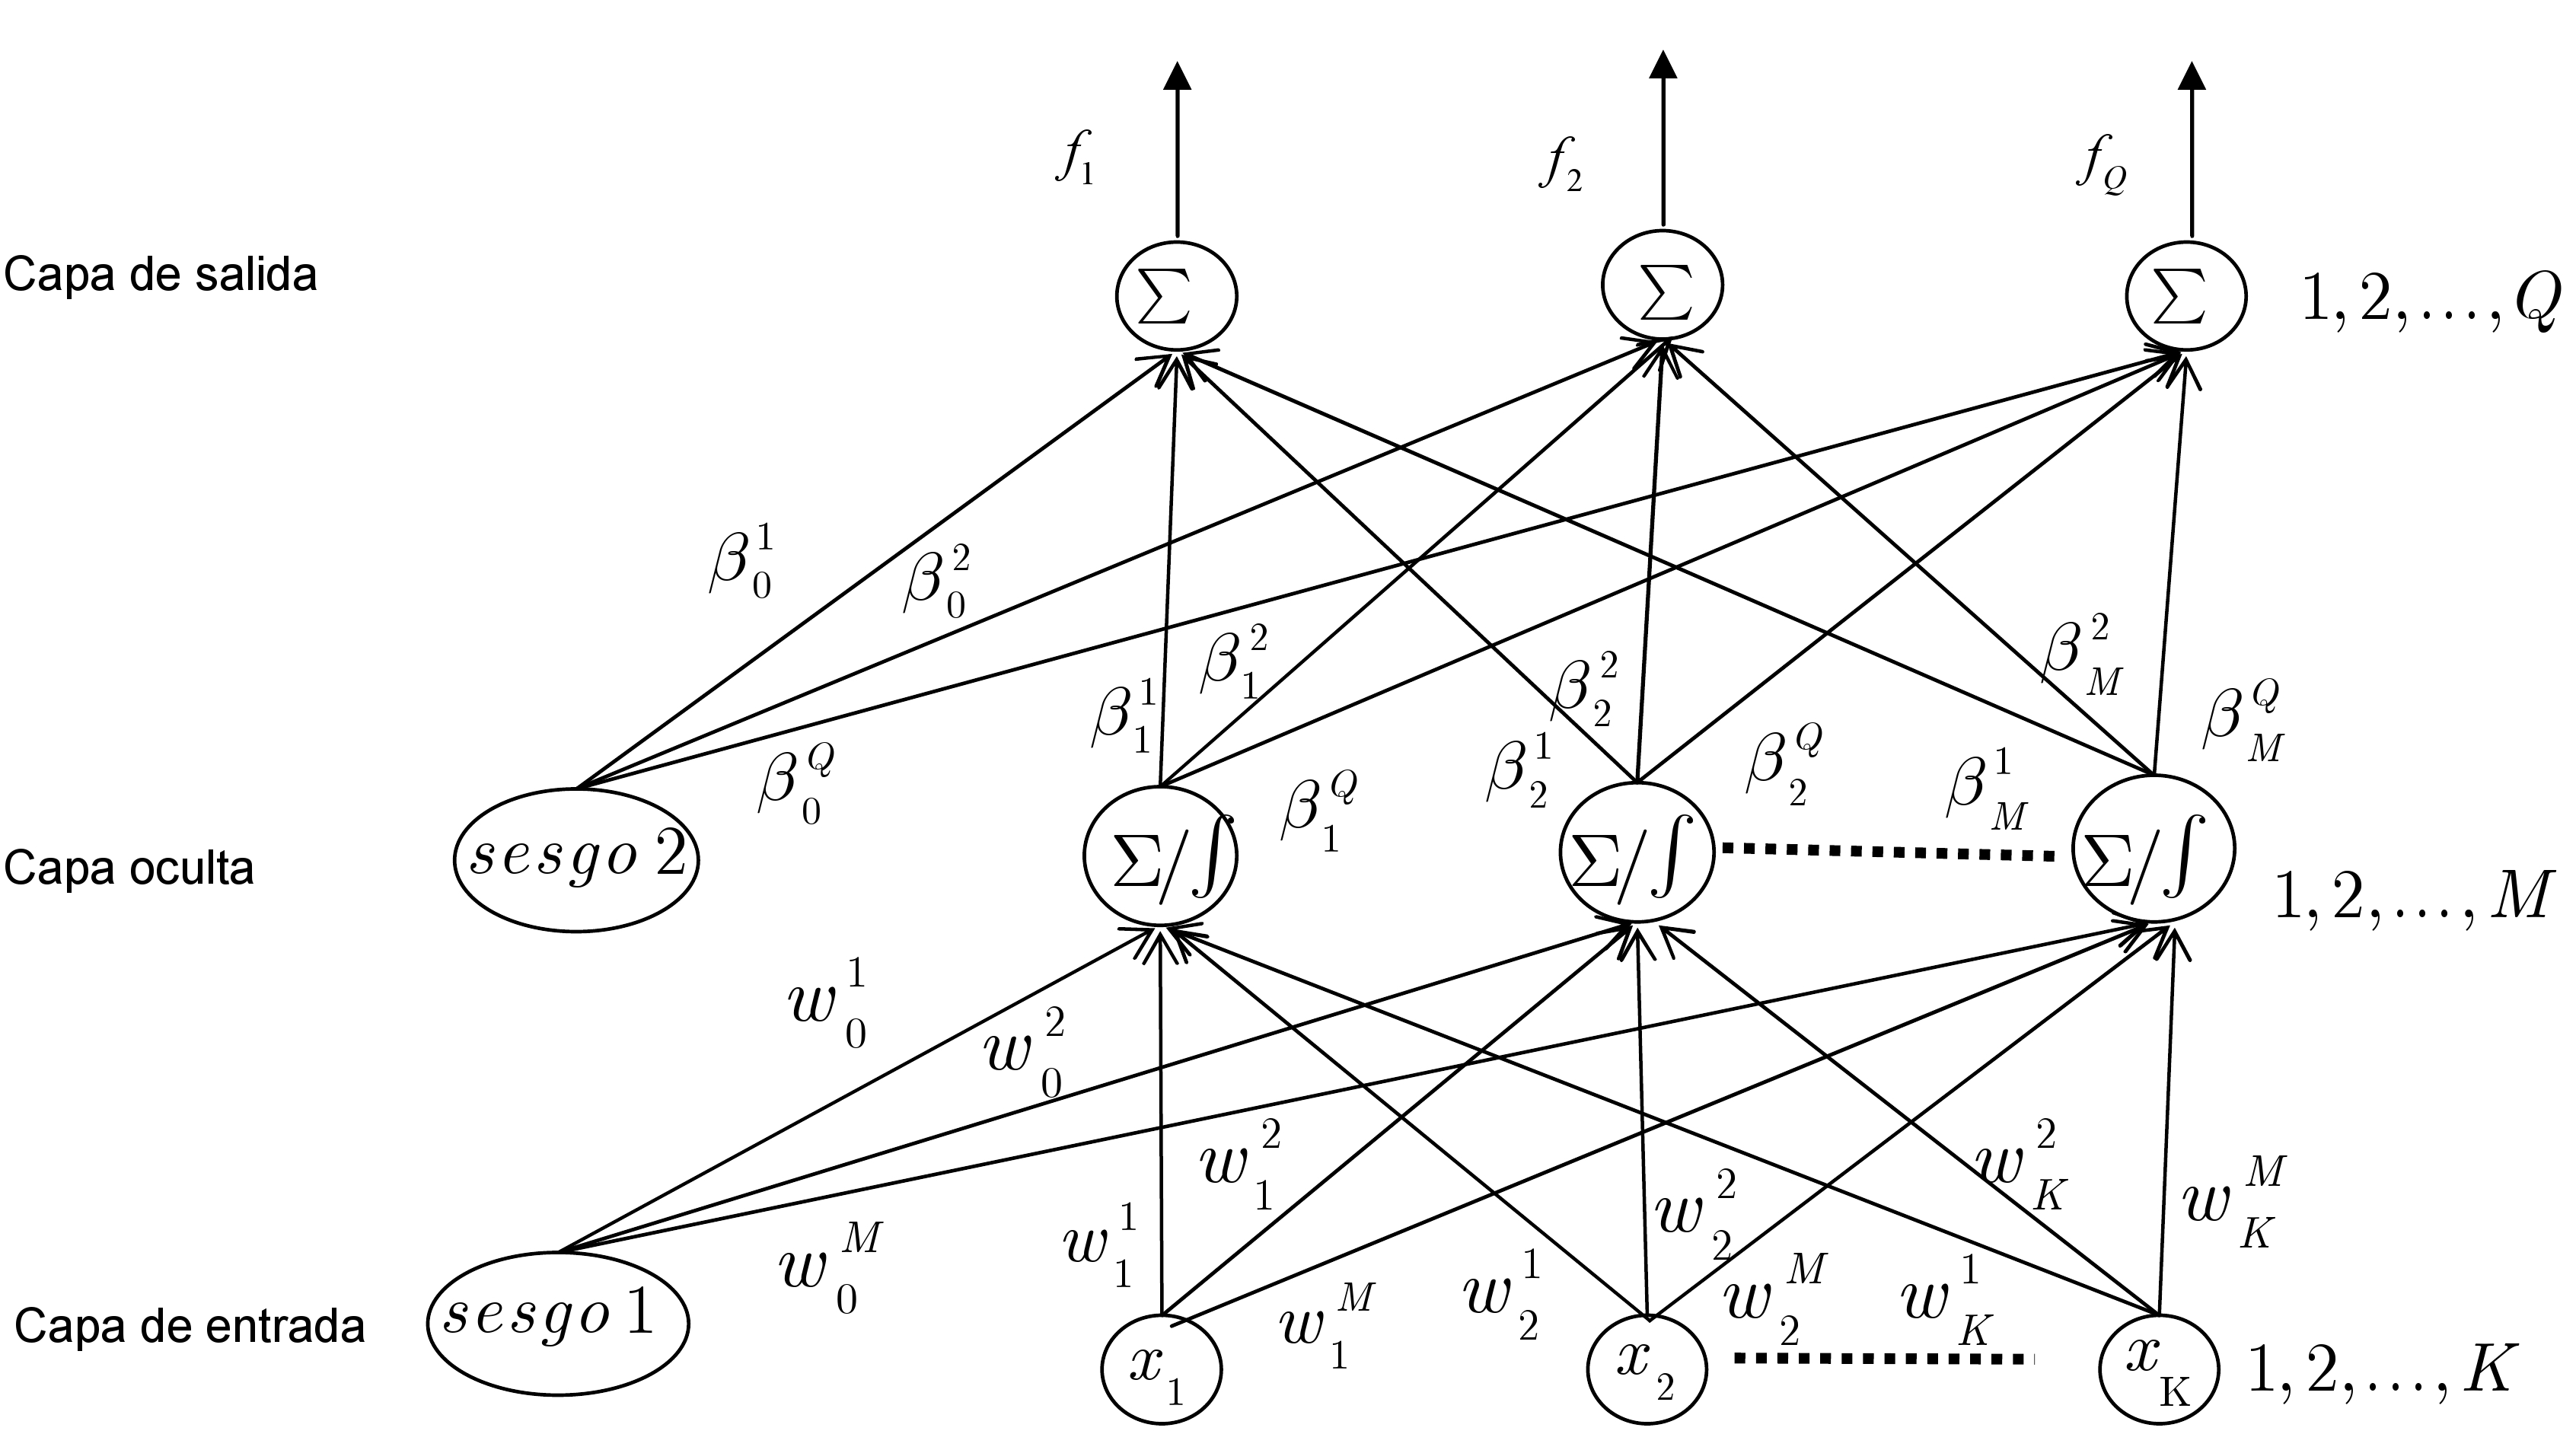
\includegraphics[keepaspectratio,width=12.5cm]{figuras/redSigmoideHaciaDelante.jpg}
\caption{Red neuronal hacia delante con unidades de base sigmoide y una capa oculta.}
\label{redSigmoideHaciaDelante}
\end{figure}

Existen  distintas  formas  de transmisión  de  la información entre los nodos de una ANN,
que determinan la naturaleza de la misma. De este modo, los tipos de transmisión son los
siguientes:
\begin{description}
	\item[Transmisión hacia delante:] Este  tipo  de transmisión  se
	produce desde los nodos de la capa de entrada	hasta los	nodos de la capa de salida.
	Las ANNs que presentan este tipo de transmisión	se
	denominan redes de transmisión hacia	delante o \textit{feedforward}.
	\item[Transmisión lateral:] Este tipo de transmisión se produce	entre nodos
	de la 	misma capa. Las	ANNs que presentan este tipo de transmisión se denominan
	redes con	transmisión lateral.
	\item[Transmisión hacia atrás:] Este tipo de transmisión	(también llamada transmisión
	\textit{feedback}) se	produce desde los nodos de la capa de salida hasta los nodos de
	la capa de entrada. Las	ANNs	que  presentan  este  tipo  de  transmisión  se
	denominan  redes  con  realimentación o redes recurrentes.
 \end{description}
En este trabajo trabajo se utilizan redes de transmisión hacia delante, con una sola
capa oculta y con unidades de base sigmoide, por su buena adaptación y resultados en
problemas de clasificación de patrones.

El modelo funcional o función de salida asociada a cada
una de las neuronas de la salida de este tipo de redes es el siguiente:
\begin{equation}\label{modelof}
	f_{q}\left(\mathbf{x},\mathbf{\Theta}_{q} \right)= \beta_{0}^q + \sum_{j=1}^M
	\beta_{j}^q B_{j} \left( \mathbf{x},\mathbf{w}_{j}\right), \quad \text{para } q=1...Q
\end{equation}
donde $Q$ es la neurona de salida $q$ de la
red (en el caso de que haya varias salidas), $\displaystyle
\mathbf{\Theta}_{q}=\left(\beta_{0}^q,\beta_{1}^q,...,\beta_{M}^q,
\mathbf{w}_{1},...,\mathbf{w}_{M}\right)$ es el vector de pesos de esa neurona
$q$,
$\displaystyle \mathbf{w}_{j}=\left( w_{0}^j,w_{1}^j,...,w_{k}^j\right) $ es el vector de
pesos de las conexiones entre la capa de entrada y la neurona de la capa oculta $j$, $M$
es el número de neuronas de la capa oculta (ver figura \ref{redSigmoideHaciaDelante}), $K$ el número
de neuronas o características en la capa de entrada (ver figura \ref{redSigmoideHaciaDelante}),
$\mathbf{x}$ el valor de las entradas de la ANN, $\displaystyle B{j}\left(
\mathbf{x},\mathbf{w}_{j}\right)$ es la función de base de la neurona $j$
de la capa oculta y $\displaystyle \beta_{0}^q$ y $\displaystyle w_{0}^j$ son los sesgos
del modelo asociado a la neurona $q$ en la capa de salida, y a la neurona $j$ de la capa
oculta respectivamente.

\section{Taxonomía}\label{taxonomia}
\noindent Se pueden considerar dos tipos fundamentales de funciones de
base o transferencia en una ANN:
\begin{description}
\item[Funciones de ventana:] Son funciones de entorno local, como pueden ser las
funciones de base radial (\textit{Radial  Basis  Functions}, RBFs).  Poseen  una  mayor
capacidad de aproximar  datos anómalos aislados, pero una mayor dificultad en entornos
globales o cuando el número de entradas es demasiado alto.
\item[Funciones de proyección:] Son funciones de entorno global, como las unidades
de base sigmoide (\textit{Sigmoidal Units}, SUs) o las  unidades de base Producto
(\textit{Product	Units}, PUs). Al ser globales, presentan dificultades en 	la
aproximación de  datos	aislados pero suelen actuar mejor en problemas donde el	número
de variables es alto.
\end{description}

En  general,  consideraremos  dos  tipos  de  modelos  de  red, en función de
la activación de las variables independientes: Modelos aditivos  y
modelos multiplicativos:
\begin{description}
	\item[Modelo aditivo:] Este modelo es el más utilizado dentro de las ANNs, y los nodos
	que componen la estructura de la red proporcionarían la siguiente salida:
	\begin{displaymath}
	B{j}\left(
	\mathbf{x},\mathbf{w}_{j}\right)=h\left(w_{0}^j+w_{1}^jx_{1}+w_{2}^jx_{2}+...+w_{n}^jx_{
	 k} \right)
	\end{displaymath}
	siendo $n$ el número de características o neuronas de entrada de la red, $w_{0}^j$ el
	sesgo del modelo asociado a la neurona $j$ y $h(.)$ la función de salida o
transferencia
	de la	neurona $j$.
	\item[Modelo multiplicativo:] Este modelo es más reciente, e   intenta  afrontar
	aquellos  casos  en	los  que  existe  una  interacción  entre  las  variables  y  las
	regiones  de decisión	que no  pueden 	separarse por hiperplanos:
	\begin{displaymath}
	B_{j}\left(\mathbf{x},\mathbf{w}_{j}\right)=
	x_{1}^{w_{1}^j}x_{2}^{w_{2}^j}...x_{n}^{w_{k}^j}
	\end{displaymath}
	Como se puede observar no existe un sesgo, pues carece de sentido para este tipo
	de modelos. La función de salida o transferencia suele ser la función identidad.
\end{description}

\subsection{Redes con unidades de base sigmoides}\label{unidadesSigmoide}
\noindent Las neuronas con SUs tienen la siguiente expresión como
función de salida o transferencia:
\begin{displaymath}
	B_{j}\left(\mathbf{x},\mathbf{w}_{j}\right)=\frac{1}{1+exp\left(-\left(w_{0}
^j+\sum_{i=1}^{K} w_{i}^{j}x_{i} \right) \right)}
\end{displaymath}

En la figura \ref{ejemploSigmoides} se muestran algunos ejemplos de funciones de base
sigmoide.

\begin{figure}[htb]
\centering
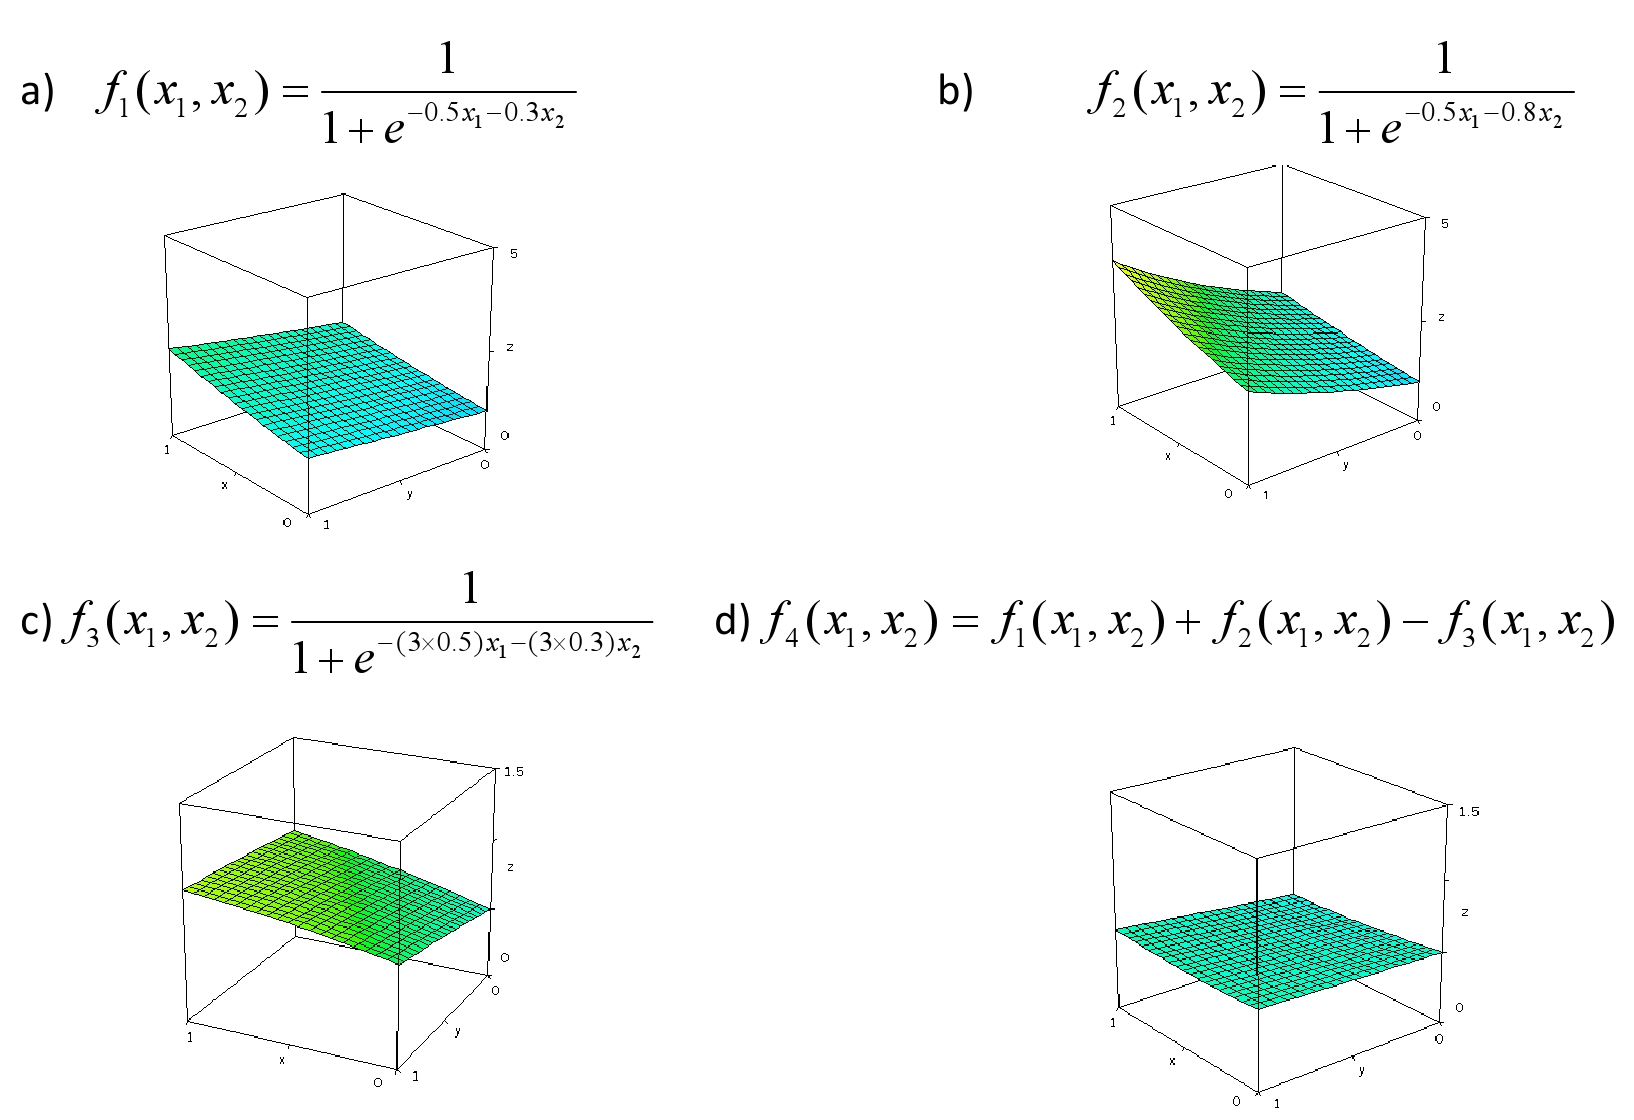
\includegraphics[keepaspectratio,width=12.5cm]{figuras/ejemploSigmoides.jpg}
\caption{Ejemplos de funciones de base sigmoide, SUs.}
\label{ejemploSigmoides}
\end{figure}

Las redes con SUs, también conocidas como perceptrón multicapa (\textit{Multi Layer
Perceptron}, MLP), poseen las siguientes propiedades:
\begin{enumerate}
	\item La familia de funciones reales que representan puede aproximar cualquier función
	continua	con  suficiente  precisión,  con  tal  de  que  el  número  de  nodos  de  la
	capa	oculta  no  esté	acotado. Se dice por tanto que son aproximadores universales.
	\item Son fáciles de entrenar, aunque se obtienen con frecuencia óptimos locales.
	\item Se obtienen modelos eficientes en entornos alisados.
	\item Son funciones acotadas.
	\end{enumerate}
En la figura \ref{redSigmoideHaciaDelante} se representa una ANN hacia delante
con unidades de base sigmoides, con una capa de entrada, una capa oculta y una capa de
salida.

\subsection{Redes con unidades de base producto}
\noindent     Las ANNs con PUs introducidas por Durbin y Rumelhart \cite{Durbin1989} en
1989, son aquellas que están formadas por nodos que siguen un modelo multiplicativo de
proyección, con la siguiente función de salida o transferencia:
\begin{displaymath}
B_{j}\left(\mathbf{x},\mathbf{w}_{j}\right)=x_{1}^{w_{1}^j}x_{2}^{w_{2}^j}...x_{n}^{
	w_{n}^j}=\prod_{i=1}^n x_{i}^{w_{i}^j}
\end{displaymath}

Entre las ventajas de las redes PU se encuentran las siguientes:
\begin{enumerate}
	\item Como consecuencia del Teorema de Stone-Weierstrass \cite{Bishop1961}, se ha
	demostrado que las
	redes PU son aproximadores universales, (obsérvese que las funciones
	polinómicas de varias variables, son un subconjunto de los modelos basados en unidades
	producto).
	\item La  posibilidad  de  usar  exponentes  negativos  permite  expresar  cocientes  y
	entre  las variables.
	\item Durbin  y  Rumelhart \cite{Durbin1989} demostraron  que  la  capacidad  de
	información  de  una
	única unidad  de tipo  producto  (medida  como  la  capacidad  para  el  aprendizaje
	de	patrones booleanos aleatorios) es aproximadamente igual a $3N$, comparado con el
	valor de	$2N$ que corresponde a una unidad de tipo aditivo, siendo $N$ el número de
	entradas de la unidad.
	\item Los  exponentes  del  modelo  son  números  reales.  Esta  característica  tiene
	especial importancia,  sobre  todo  si  se  tiene  en  cuenta  que  son  frecuentes
	las	situaciones  en  el modelado de datos reales en las que, la relación entre las
	variables	responde a una estructura de  tipo  potencial,  donde  las  potencias  no
	están	restringidas  a  los  números naturales  o enteros.
	\item Permiten  implementar  funciones  polinómicas  de  orden  superior.  Han
	demostrado	buenos resultados en el modelado de datos en los que existen interacciones
	de diferentes	órdenes entre  las  variables  independientes  del  problema.  De  esta
	forma,	cuando existen interacciones  entre  las  variables  que  intervienen  en  un
	determinado  fenómeno, las  ANNs basadas en PUs permiten obtener modelos
	más simplificados que las ANNs de tipo sigmoide.
	\item Junto a esto, es posible obtener cotas superiores de la dimensión
	de \textit{Vapnik-Chervonensky} (VC), para redes basadas en PUs similares a las
	conocidas para las	redes SUs, lo que supone que poseen una capacidad de
	generalización similar.
	\item A diferencia de lo que ocurre con las redes SUs o RBFs,
	las	funciones derivadas parciales del modelo obtenido a partir de una red PU
	son funciones	del   mismo tipo. Este hecho ayuda con frecuencia al estudio de las
	tasas de cambio de la   variable dependiente  del  modelo  con  respecto  a  cada  una
	de  las  variables independientes.
\end{enumerate}

Como  contrapartida,  las  ANNs  con  PUs  presentan  un  inconveniente
importante:

La  superficie  de error  asociada  es  especialmente  compleja,  con  numerosos  óptimos
locales  y regiones  planas,  y  por tanto  con  mayor  probabilidad  de  quedar  atrapado
en  alguno \cite{Ismail2000}.  La  estructura potencial  del  modelo provoca  que
pequeños cambios en los exponentes  tengan  como  consecuencia  un cambio significativo
en los  valores  de la  función  y  en  la  función  de  error.  Así, los  algoritmos  de
entrenamiento de redes basados en el gradiente quedan con frecuencia, y de forma especial
en este tipo de ANNs, atrapados en óptimos locales. Esta dificultad
relacionada con
el entrenamiento, es una de las razones por las que, a pesar de las ventajas anteriormente
señaladas, la teoría de ANNs basadas  en  PUs  ha  tenido  poco
desarrollo,  y  han  sido  menos utilizadas  como modelos para problemas de
clasificación y de regresión que otros tipos de ANNs.

En la figura \ref{ejemploProducto} se muestran algunos ejemplos de funciones de base
producto.

\begin{figure}[htb]
\centering
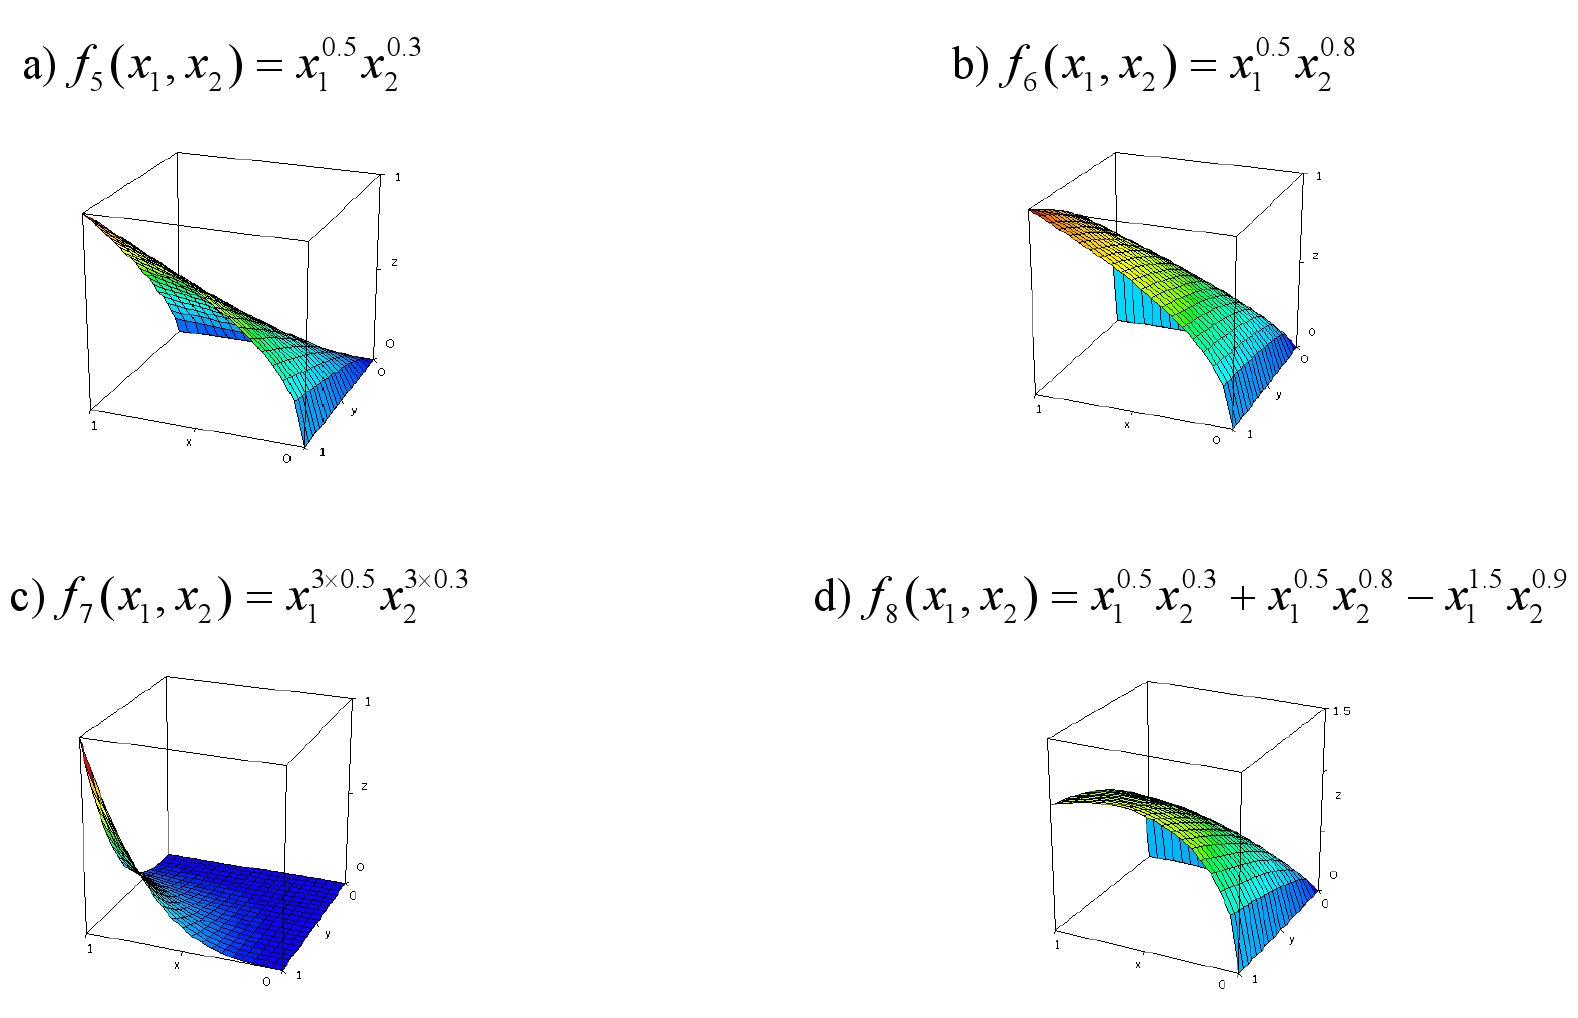
\includegraphics[keepaspectratio,width=12.5cm]{figuras/ejemploProducto.jpg}
\caption{Ejemplos de funciones de base producto, PUs.}
\label{ejemploProducto}
\end{figure}

\subsection{Redes con unidades de base radial}
\noindent     Los nodos ocultos de las ANNs con RBFs presentan funciones de activación de
tipo ventana.  Cada uno  de  los  nodos  RBF  realiza  una
aproximación local  independiente del  espacio  de búsqueda,  normalmente  mediante  una
campana  de Gauss.  La  capa  de  salida  de  tipo lineal  auna  el efecto  independiente
de  cada nodo,  sumando  cada  valor  obtenido.  La  idea  es  que cada  nodo  esté
situado en un entorno del espacio de búsqueda formado por las variables de entrada y
además con un radio determinado. El proceso de aprendizaje de la red de RBFs consistirá en
ir moviendo dichos nodos a lo largo del espacio de búsqueda, modificando los centros y los
radios de los mismos, para ajustarlos de la mejor forma a los datos de entrenamiento.

La  función  de  activación  será  equivalente  a  la  función  de  distancia
euclídea  (tomando  como centro de la RBF el vector $\mathbf{w}_{j}$), y la
función de
transferencia será una función de tipo Gaussiano. Por tanto, la función de
salida o transferencia sería la siguiente:
\begin{displaymath}
B_{j}\left(\mathbf{x},\mathbf{w}_{j}\right)=
e^{-\frac{1}{2}\left( \frac{d\left( \mathbf{x},\mathbf{w}_{j}\right) }{r_{j}}\right) }
\end{displaymath}
siendo
\begin{displaymath}
	d\left( \mathbf{x},\mathbf{w}_{j}\right) =\lVert
	\mathbf{x}-\mathbf{w}_{j}\rVert=\sqrt{\sum_{i=1}^n \left( x_{i}-w_{ij}\right)^2 }
\end{displaymath}
siendo $w_{ij}$ el peso asociado a la neurona $j-esima$ de la capa oculta y la neurona
$i-esima$ de la capa de entrada.

Algunas de las características de las redes RBF son:
\begin{enumerate}
		\item Se ha demostrado que las ANNs con unidades RBF son aproximadores
		universales \cite{Park1991}.
		\item En comparación con las redes MLP, las redes RBF presentan la
		ventaja de que	cada nodo en la capa oculta es un elemento local en el modelo, lo
		que hace que para	un	determinado patrón sólo algunas unidades ocultas se activen.
		Esta característica	facilita	el entrenamiento, disminuyendo el número de óptimos
		locales y regiones	planas de la superficie de error, al desaparecer gran parte
		de las	interacciones entre los pesos.
		\item Por último, el proceso de entrenamiento de una red MLP consta
		de una sola etapa, mientras que las redes RBF suelen entrenarse en dos etapas,
		siendo las	funciones	de base aproximadas en primer lugar mediante técnicas de
		aprendizaje no supervisado, determinando los centros y el número de funciones de
		base mediante, por ejemplo, un algoritmo $k$-medias,  y los	pesos	entre las capas
		oculta y de salida en segundo lugar,	mediante métodos supervisados.
\end{enumerate}

En la figura \ref{ejemploRadial} se muestra un ejemplo gráfico de la superficie generada
por el efecto aditivo de tres neuronas \textit{RBF}.
\begin{figure}[htb]
\centering
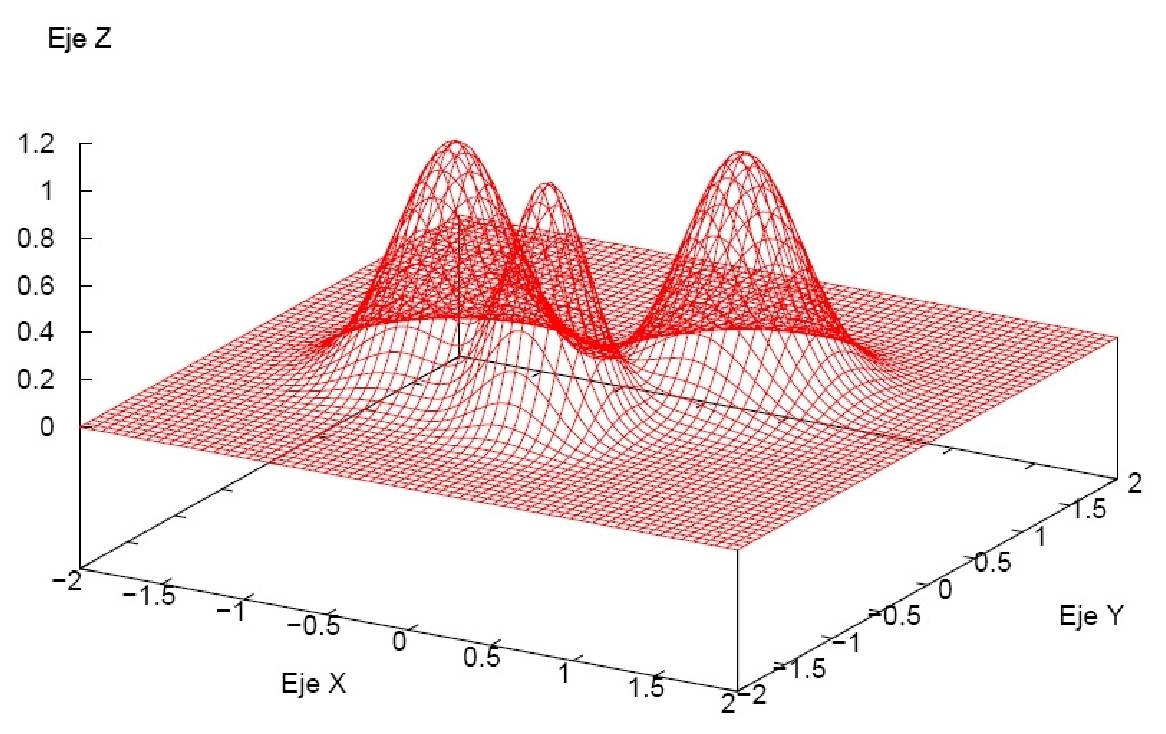
\includegraphics[keepaspectratio,width=12.5cm]{figuras/ejemploRadial.jpg}
\caption{Ejemplos de funciones de unidad de base radial, RBF.}
\label{ejemploRadial}
\end{figure}

\subsection{Redes híbridas}\label{redesHibridas}
\noindent Hasta este momento las ANNs que hemos definido poseían un solo tipo de
unidad de base como nodos de la red en la capa oculta, ya fuesen SUs, PUs o RBFs.

La combinación de diferentes funciones de base en capa oculta puede tener varias
ventajas si se consideran tareas de clasificación que tienen áreas generalmente
separadas, pero en las cuales es difícil situar su borde de decisión, debido a que las
mejores funciones discriminantes para cada clase del problema pueden ser muy diferentes.
Una mixtura de unidades de base puede proporcionar bordes de decisión flexibles,
cubriéndose las desventajas que puedan tener el uso de modelos con un solo tipo de unidad
de base o modelos puros. Donoho \cite{Donoho1989} demostró que cualquier función continua
se puede descomponer en dos tipos de funciones mutuamente excluyentes, una función
asociada con funciones de tipo proyección, SUs o PUs, y la otra asociada con funciones de
tipo ventana, RBFs. A pesar de
ello, en la práctica, es difícil separar las diferentes
localizaciones de una función y estimar la función residual mediante una aproximación
funcional basada en proyecciones, sin quedar atrapado en óptimos locales en la
minimización del error \cite{Friedman1991}.

Varios autores han propuesto la hibridación de redes con diferentes funciones de base, ya
sea con una sola capa oculta híbrida o interconectando varias capas puras. De acuerdo a
Duch y Jankowski \cite{Duch2001}, la hibridación de diferentes funciones de transferencia
dentro de una ANN se puede hacer de dos maneras. Una de ellas sería utilizar un método
constructivo que seleccione la mejor función de base a partir de un conjunto de funciones
RBF candidatas \cite{Duch2001a}; y un segundo método
sería partir de redes con diferentes unidades de base, y usar técnicas de poda o de
regularización para reducir el número de funciones \cite{Duch2001, Jankowski2001}.

Pao \cite{Pao1992} presentó una combinación de varias funciones (polinómicas, periódicas,
sigmoidales y gaussianas) en lo que llamó redes de enlace funcional (\textit{Functional
Link Networks}). La idea consistía en el uso de enlaces funcionales, añadiendo
transformaciones no lineales de las variables de entrada al conjunto original de variables,
y suprimiendo la capa oculta, haciendo una la primera aproximación no lineal fija, y una
segunda aproximación adaptativa.

Una aproximación más compleja considera varias capas o modelos, cada una conteniendo una
estructura de funciones de base, dando como resultado un sistema modular. Por ejemplo,
Iulian
\cite{Iulian2002} propuso una metodología incluyendo tres módulos distintos, implementando
una ANN hacia delante (llamada red neuronal RBF de tipo gaussiana), un proceso de
análisis de componentes principales, y una red SU. Otra
propuesta, de Lehtokangas and Saarinen \cite{Lehtokangas1998}, considera dos capas ocultas
en el modelo, la primera compuesta por funciones gaussianas y la segunda por SUs.

Las ANNs que utilizan diferentes funciones de base deberían contener
menos nodos, permitiendo que la función desempeñada por la red sea
más transparente. Por ejemplo, un hiperplano se puede utilizar para dividir
un espacio de entrada en dos clases y una función adicional de Gauss
que tenga en cuenta cualquier anomalía local. El análisis de la aproximación realizada
por una red MLP entrenada con los mismos datos no es tan simple. En este contexto cabe
señalar el trabajo de Cohen e Intrator \cite{Cohen2002a}, que se basa en las propiedades
de dualidad y complementariedad de las funciones de tipo proyección y de tipo ventana.

Recientemente, Wedge \cite{Wedge2006} presentó una ANN
híbrida compuesta por unidades de base RBFs y SUs. Se utiliza un algoritmo de
entrenamiento en tres pasos, en el cual se intentan identificar los aspectos de
una relación funcional que son expresados separadamente de aquellos que varían solo dentro
de las regiones particulares del espacio de entrada.

En \cite{Kordik2010}, se propone un algoritmo evolutivo llamado \textit{GAME} para la
optimización de la topología de una ANN, combinando diferentes tipos de neuronas,
entrenadas dentro de la red mediante varios algoritmos de optimización y principios de
meta-aprendizaje, para construir finalmente una ANN supervisada hacia delante con varias
capas y con varias funciones de base por capa.

Otros autores como Hervás \cite{Hervas2007,Hervas2007a}, hacen uso de
un AE que utiliza la función de entropía cruzada para evaluar a los
individuos de la población. Dicha población se compone de ANNs híbridas con una sola
capa oculta compuesta por unidades de tipo PUs y SUs. El algoritmo se encarga
de evolucionar simultáneamente la arquitectura y los pesos de cada red, utilizando un
operador de mutación adaptado a cada tipo de unidad de base. Los resultados
reflejan que la hibridación puede ser una alternativa viable con respecto a los
modelos puros en determinados problemas, y deja abiertas algunas cuestiones sobre
la posibilidad de crear procedimientos que permitan elegir
entre diferentes familias de funciones durante la evolución de las ANNs.
En \cite{Gutierrez2007,Gutierrez2009} se realiza una mejora del método anterior,
mediante la inclusión de un procedimiento de doble elitismo en el algoritmo evolutivo, y se da
 la posibilidad de utilizar tres tipos diferentes de redes, en función del tipo de
unidades de base usadas, redes Producto-Sigmoide (PSU), Producto-RBF (PRBF),
Sigmoide-RBF (SRBF). Algunas conclusiones de este trabajo
muestran que la elección adecuada del tipo de base a utilizar depende fuertemente del
conjunto de datos a clasificar, pero que, en general, los modelos compuestos por SUs y RBFs
consiguen un rendimiento mayor que los compuestos por SUs y PUs, especialmente en aquellos
conjuntos de datos con dos clases, donde solamente existe una función discriminante.
También se comprueba empíricamente que los modelos formados por SUs y PUs no consiguen una
precisión mayor que los restantes tipos de hibridación, aunque si consiguen tener un menor
número de conexiones, permitiendo que sean más interpretables.

A continuación, presentamos el modelo funcional o función de salida de una red
neuronal formada por diferentes tipos de unidades de base en su capa oculta (ver figura
\ref{ejemploHibrida}):
\begin{equation}\label{modelofhibrido}
f_{q}\left(\mathbf{x},\mathbf{\Theta}_{q} \right)= \alpha_{0}^q +\sum_{j=1}^{m1}
B_{j}^q \sigma_{j} \left( \mathbf{x},\mathbf{u}_{j}\right)+\sum_{k=1}^{m2}
\beta_{k}^q B_{k} \left( \mathbf{x},\mathbf{w}_{k}\right),
\end{equation}
donde $q$ es el número de unidades, nodos o neuronas de salida de la red,
$\displaystyle
\mathbf{\Theta}_{q}=\left(\alpha_{0}^q,\alpha_{1}^q,...,\alpha_{m1}^q,\beta_{0}^q,\beta_
{1}^q,...,\beta_{m2}^q,\mathbf{u}_{1},...,\mathbf{u}_{m1},
\mathbf{w}_{1},...,\mathbf{w}_{m2} \right)$ son los vectores de pesos de la neurona de
salida $q$, $\displaystyle \mathbf{u}_{j}=\left( u_{0}^j,u_{1}^j,...,u_{K}^j\right) $ y
$\displaystyle \mathbf{w}_{k}=\left( w_{0}^k,w_{1}^k,...,w_{K}^k\right) $ es el vector de
pesos de las conexiones entre la capa de entrada y la neurona oculta $j$ y $k$, $m1$ es el
número de neuronas ocultas del tipo 1 y $m2$ el el número de neuronas ocultas del tipo 2,
$K$ el número de neuronas o características en la capa de entrada,
$\mathbf{x}$ el valor de las entradas de la ANN, $\displaystyle B_{j}
\left( \mathbf{x},\mathbf{u}_{j}\right)$ es la función de base de la neurona $j$ de tipo 1
, $\displaystyle B_{k}
\left( \mathbf{x},\mathbf{w}_{k}\right)$ es la función de base de la neurona $k$ de tipo 2
y $\displaystyle \alpha_{0}^q$ y $\displaystyle u_{0}^j$ son los sesgos del modelo
asociado a la neurona $q$ en la capa de salida y a la neurona $j$ en la capa oculta
respectivamente.

\begin{figure}[htb]
\centering
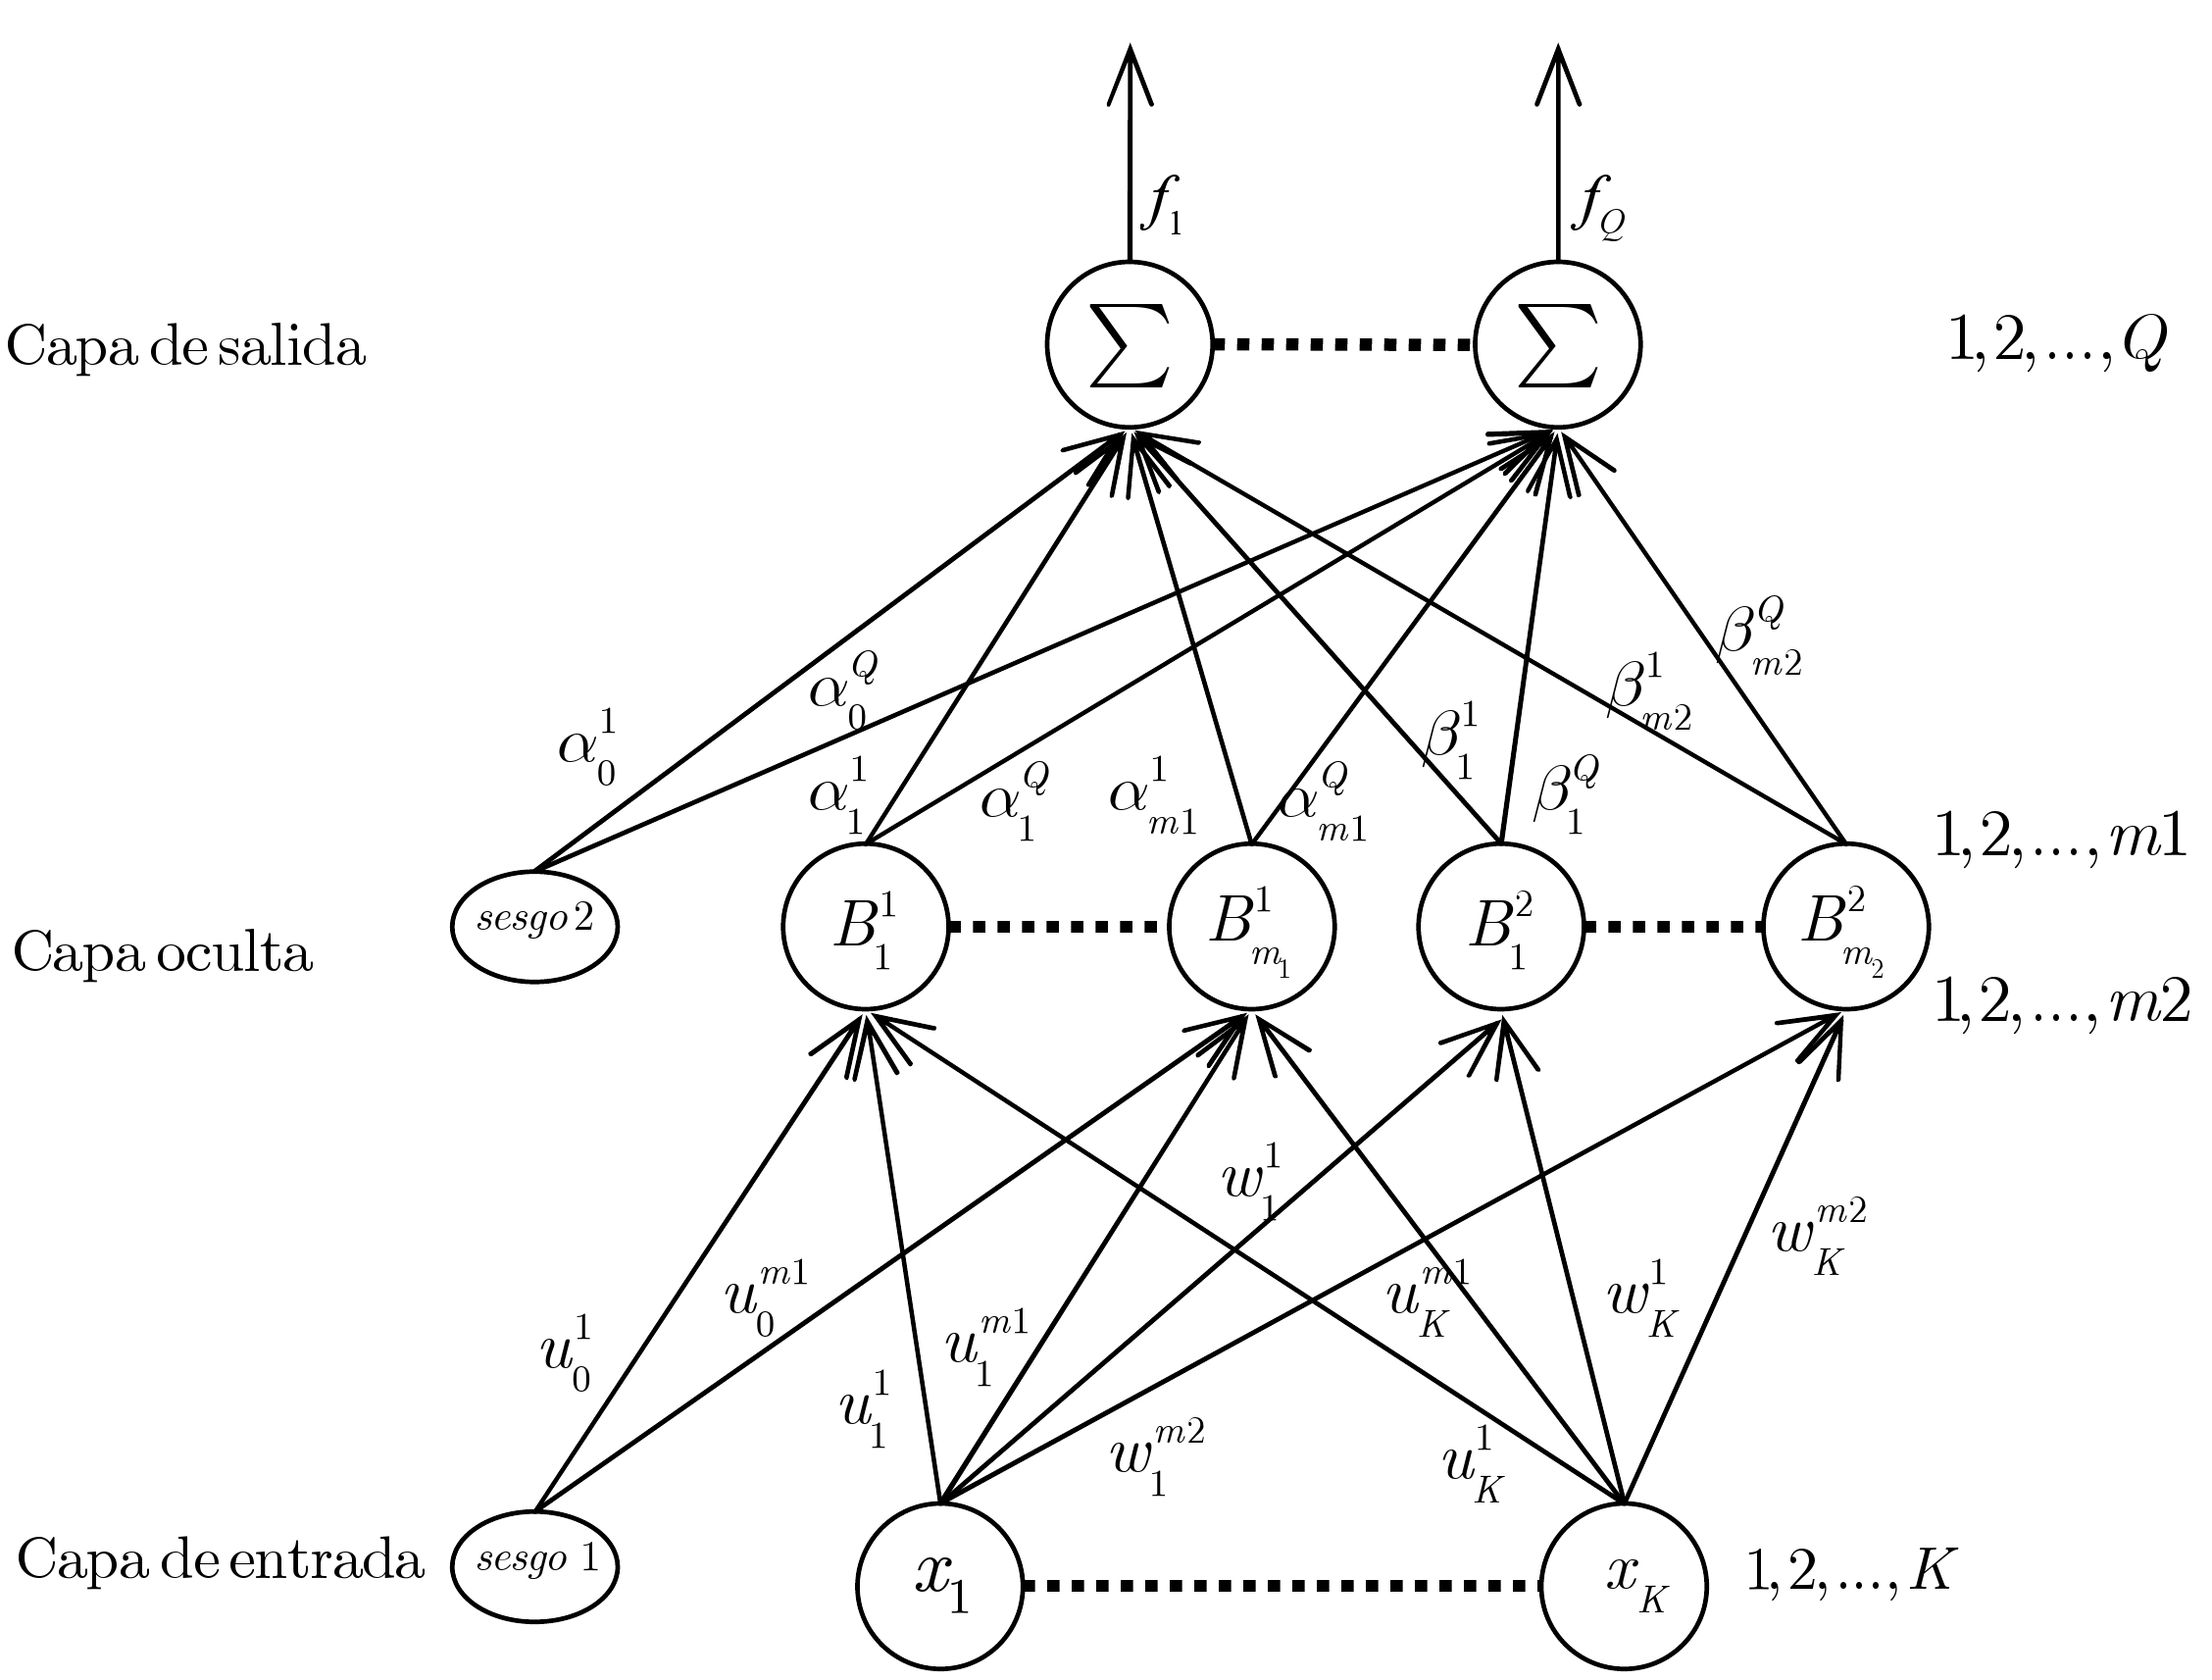
\includegraphics[keepaspectratio,width=12.5cm]{figuras/redHibridaHaciaDelante.jpg}
\caption{Red híbrida hacia delante con dos tipos diferentes de funciones de base en capa
oculta.}
\label{ejemploHibrida}
\end{figure}

% COGER EL PAPER DE NEUROCOMPUTING PARA METER LA TEORIA y el MODELO FUNCIONAL DE SALIDA
% TAMBIEN COGER EL DEL MAEB ``2007_maebA.PDf
\newpage
\section{Métodos de entrenamiento}\label{metodosEntrena}
A continuación se expone brevemente una visión global de los
métodos clásicos de optimización utilizados para el entrenamiento de ANNs, y de los
métodos que incorporan algún tipo de heurística o técnica para mejorar el aprendizaje
\cite{Kordik2010}.

\subsection{Métodos clásicos}\label{mClasicos}
\noindent La mayoría de los métodos clásicos utilizados para el entrenamiento de
ANNs tienen el problema de que pueden llegar a estancarse en una
solución que no sea lo suficientemente idónea para el problema que se
esté intentando resolver. Los métodos más comunes son:
\begin{description}
\item[Métodos constructivos:] Los métodos constructivos comienzan con una red mínima y
van añadiendo nodos y conexiones hasta que ésta es capaz de resolver el problema planteado
con una determinada precisión. Lo que se hace es adaptar el tamaño de la red al problema
en cuestión, teniendo la ventaja de que no se necesita hacer una estimación “a priori” del
tamaño de la misma, pero se necesita un experto con suficiente experiencia y un proceso de
prueba y error \cite{Burgess1994,Setiono1995}. Este tipo de métodos son susceptibles
de caer en mínimos locales \cite{Angeline1994}, además de que solo pueden llevar a cabo la
búsqueda en subconjuntos reducidos del espacio de las posibles
topologías.
\item[Métodos destructivos o de poda:] Los métodos destructivos o de poda
\cite{Reed1993,Reed1999} parten de una red suficientemente grande (inicialmente puede
sobre-entrenar y ser demasiado compleja), y sucesivamente se van eliminando nodos y
conexiones hasta llegar a una topología en la que la eliminación de un nodo no mejore los
resultados. La ventaja de estos métodos es que las redes se que obtienen son pequeñas y por
lo tanto más fáciles de implementar y entrenar. De nuevo, es primordial la experiencia del
diseñador, y se necesita un proceso de prueba y error.
\item[Métodos basados en gradiente:] El algoritmo de retropropagación
(\textit{BackPropagation}, BP) \cite{Chauvin1995} y sus múltiples variantes
\cite{Hush1993,Moller1993,Chauvin1995}
(ver siguiente sección) es uno de los más carismáticos y utilizados dentro de los métodos
basados en gradiente. Este tipo de metodologías tienen como principal inconveniente el
poder caer en óptimos locales y quedar estancado el proceso de aprendizaje, por lo que es
necesario establecer
de antemano una serie de parámetros, como por ejemplo la tasa de aprendizaje, la
inicialización de los pesos (influye en la rapidez del aprendizaje y en que se alcance o
no el mínimo global de la función de error), número de capas ocultas y número de neuronas
en cada capa, entre otros.
\end{description}

Los algoritmos clásicos suelen presentar una serie de problemas \cite{Angeline1994,
Yao1999}:
\begin{enumerate}
\item Imposibilidad de calcular el gradiente cuando la función de activación no es
derivable.
\item Incapacidad de encontrar un mínimo global si la función de error es multimodal
y/o no diferenciable.
\item Ausencia de convergencia de los algoritmos clásicos de entrenamiento cuando el
número de dígitos utilizados para representar la
función de activación o los pesos de la red (precisión) no es suficientemente grande.
\item Tendencia, por parte de los algoritmos de entrenamiento, a obtener excesivas
soluciones no óptimas en cada ejecución.
\item En general, los métodos constructivos y destructivos limitan las arquitecturas
disponibles. En algunos de éstos métodos, una vez se ha explorado una arquitectura y se ha decidido
que es insuficiente, se adopta una nueva arquitectura,
de manera que las antiguas arquitecturas se convierte en inalcanzables. Además, los
algoritmos constructivos y destructivos basan su estudio en subconjuntos topológicos,
en lugar de basarse en la clase completa de las arquitecturas de red. En consecuencia,
estos	algoritmos tienden a optimizar una clase de arquitectura en lugar de ajustar una
arquitectura apropiada para un problema determinado.
\item Las deficiencias de los métodos constructivos y destructivos se derivan de
métodos 	inadecuados para la asignación de los componentes estructurales
de una red. Se asumen que las restricciones topológicas limitan la complejidad de las
interacciones	estructurales y paramétricas, e incrementan la probabilidad de
encontrar una red suficiente buena para resolver el problema, pero lo ideal sería que
esas restricciones proviniesen de la tarea o problema en si, y no que estuvieran
implícitas en el algoritmo.
\item Otros métodos usan una sola modificación estructural predefinida, como añadir una
unidad completamente conectada en capa oculta, para generar topologías sucesivas.
Tales métodos como la escalada en colina estructurada (\textit{Structural Hill
Climbing}), son susceptibles de quedar atrapados en óptimos locales estructurales, y
hacen recaer la carga de la tarea de inducción principalmente en la
identificación de los valores adecuados de los parámetros, en vez de distribuir
la carga uniformemente.
\end{enumerate}

\subsection{Métodos heurísticos}\label{redesheuristicas}
\noindent La utilización de métodos de naturaleza heurística
\cite{Walczak1999,Abraham2000,Glover2003} para el entrenamiento de ANNs surge
en la década de  los  90  como  solución a los  problemas  de  entrenamiento presentados
por los algoritmos clásicos. A continuación se citan algunos de los métodos heurísticos
utilizados con más frecuencia para el aprendizaje de ANNs:
\begin{itemize}
	\item Variantes heurísticas de la retropropagación del error
	\cite{Riedmiller1994}, BP con velocidad adaptativa y/o optimización de
	los parámetros de aprendizaje \cite{Zainuddin2005}, la regla \textit{delta-delta} o la
	regla	\textit{delta-bar-delta} \cite{Jacobs1988}, algoritmo \textit{Quikprop}
	\cite{Veitch1991}, algoritmo \textit{iRprop+} \cite{Igel2000}.
	\item Algoritmos de gradiente conjugado como el \textit{FRCG} de Fletcher-Reeves
	\cite{Fletcher1964}, el \textit{PRCG} de Polak-Ribiére  \cite{Polak1969}
	o	el	de Powell-Beale \cite{Powell1977}.
	\item Algoritmos de tipo \textit{Quasi-Newton} como el \textit{DFP} de
	Davidon-Fletcher-Powell	\cite{Davidon1991} y el
	\textit{BFGS} de Broyden-Fletcher-Golfarb-Shannon	\cite{Broyden1970}.
	\item Algoritmos que modifican el método \textit{Quasi-Newton} como el \textit{LM} de
\\
	Levenberg-Marquard \cite{Marquardt1963}.
	\item Métodos heurísticos no basados en gradiente como el enfriamiento simulado
	(\textit{Simulated Annealing} , SA), la búsqueda  tabú (\textit{Tabu Search}, TS), la
	búsqueda dispersa (\textit{Scatter Search}, SS),
	los enjambres de partículas (\textit{Particle Swarm}, PS) y los algoritmos evolutivos
	(\textit{Evolutionary Algorithms}, EAs), siendo éstos últimos los que más impacto han
	tenido en el diseño de ANNs.
	Este	tipo de heurísticas se han utilizado muy frecuentemente para el	aprendizaje en
	ANNs \cite{Kordik2010,Alba2006}.
\end{itemize}

\paginavaciacompleta